% !TEX root = ./main.tex

\documentclass{article}
\usepackage[utf8]{inputenc}
\usepackage[ngerman]{babel}
\usepackage{pdfpages}
\usepackage{graphicx}
\usepackage{amsmath}
\graphicspath{ {./img/} }

\usepackage{lipsum}
\usepackage{float}
\usepackage{listings}

\usepackage{xcolor}

\definecolor{codegreen}{rgb}{0,0.6,0}
\definecolor{codegray}{rgb}{0.5,0.5,0.5}
\definecolor{codepurple}{rgb}{0.58,0,0.82}
\definecolor{backcolour}{rgb}{0.95,0.95,0.92}

\lstdefinestyle{mystyle}{
    backgroundcolor=\color{backcolour},   
    commentstyle=\color{codegreen},
    keywordstyle=\color{magenta},
    numberstyle=\tiny\color{codegray},
    stringstyle=\color{codepurple},
    basicstyle=\ttfamily\footnotesize,
    breakatwhitespace=false,         
    breaklines=true,                 
    captionpos=b,                    
    keepspaces=true,                 
    numbers=left,                    
    numbersep=5pt,                  
    showspaces=false,                
    showstringspaces=false,
    showtabs=false,                  
    tabsize=2
}

\lstset{style=mystyle}
\lstset{literate=%
{Ö}{{\"O}}1
{Ä}{{\"A}}1
{Ü}{{\"U}}1
{ß}{{\ss}}2
{ü}{{\"u}}1
{ä}{{\"a}}1
{ö}{{\"o}}1
}

\newcommand{\nr}{1}


\title{Aktorik Sensorik \\ Labor 1}
\author{Anton Kress (S872899), Jan Abel (S876662)}
\date{October 2020}

\begin{document}

\maketitle

\newpage
\tableofcontents 
\section{Labor 1}

\subsection{Einleitung und Ziel}

Um später einen permanent erregten Gleichstrommotor zu modellieren, soll
in dieser ersten Laborübung in Aktor und Sensorik die wichtigsten
Kennwerte des Systems bestimmt werden. Dieses sind die Momentenkonstante
$k_M$, der Ankerwiderstand $R$, die Motorkonstante $k_e$ und der
Verstärkungsfaktor $A$ des Messverstärkers. 

Um diese Konstanten zu bestimmen wurden jeweils eine Menge an Messwerten
aufgenommen. Mit diesen wird mittels der Methode der kleinsten Quadrate 
Ausgleichsrechnungen durchgeführt. Dadurch erhalten wir eine lineare
Funktionen aus denen sich die gesuchten Konstanten bestimmen lassen.
\subsection{Grundlagen und Theorie}

\subsubsection{Methode der kleinsten Quadrate}
Die Methode der kleinsten Quadrate ist ein mathematisches Verfahren, bei dem eine lineare Regression
auf der Basis einer Wolke aus Datenpunkten berechnet werden soll. Es soll eine Kurve gefunden werden,
die möglichst nah an den Punkten verläuft. Dazu bestimmt man die Parameter dieser Kurve numerisch, indem die Summe 
der quadratischen Abweichungen der Kurve von den beobachteten Punkten minimiert wird.

Zur Umsetzung der Methode der kleinsten Quadrate in Matlab werden die Funktionen polyfit() und polyval() verwendet. 
polyfit() erhält beim Aufruf die Werte der Punktwolke sowie den Grad des Polynoms und gibt die entsprechenden Koeffizienten
zurück. polyval() ermittelt aus den Koeffizienten und den x-Werten die tatsächlichen Werte, mit welchen die Kurve geplottet 
werden kann. 

\subsubsection{Inkrementalgeber}
Ein Inkrementalgeber ist ein Messinstrument zur Ermittlung von Lage- oder Winkeländerung (bei rotierenden Objekten). 
Als verschiedene Arten wird zwischen der photoelektrischen Abtastung (entweder als abbildendes oder interferentielles
Messprinzip), der magnetischen Abtastung und per Schleifkontakt unterschieden. Dabei werden zwei um 90 Grad verschobene
Signale erzeugt, über die sich Drehgeschwindigkeit, -richtung und -winkel bestimmen lassen.
Im Beispielt der photoelektrischen Abtastung wird eine Drehscheibe verwendet, die mit mehreren Schlitzen unterteilt ist und 
zwischen einer Leuchtdiode und zwei leicht versetzten Photodetektoren angebracht ist. Wenn sich die Scheibe dreht, zählen
die Photodetektoren die Impulse, welche von Leuchtdiode und Lichtgitter der Drehscheibe entstehen.  
\subsection{Aufgabenstellung und Versuch}

\subsubsection{Messung des Stillstandsdrehmomentes}

Im ersten Versuch soll die Momentenkonstante $k_m$ bestimmt werden.
Sie hängt folgendermaßen mit dem Drehmoment $M_M$ und dem Motorstrom $i_a(t)$
zusammen. 

\begin{equation} \label{eq111}
    \begin{split}
        M_M(t)&=k_m \cdot i_a(t)\\
        k_m&=\frac{M_M(t)}{i_a(t)}
    \end{split}
\end{equation}

Als Messwerte ist eine Matrix mit den Motorströmen $I_a$ und der Auslenkungskraft $F$
gegeben. Um daraus das Drehmoment $M_M$ zu bestimmen wird der Radius $r$ benötigt,
welcher mit $1 \mathrm{cm}$ gegeben ist.

\begin{equation} \label{eq112}
    \begin{split}
        M_M&=r \cdot F \\
        k_m&=\frac{r\cdot F(t)}{i_a(t)}
    \end{split}
\end{equation}

Anschließend kann die Momentenkonstante $k_m$ über die Steigung der geplotteten
Gerade bestimmt werden. Hierfür muss gewährleistet werden, dass der Arbeistpunkt
linear ist. Deshalb dürfen die letzten drei Messwerte in der linearen Regression
nicht betrachtet werden.

\begin{equation} \label{eq113}
    \begin{split}
        k_m\simeq 0.022 \mathrm{\frac{Nm}{A}}
    \end{split}
\end{equation}

\begin{figure}[H]
 \centering
 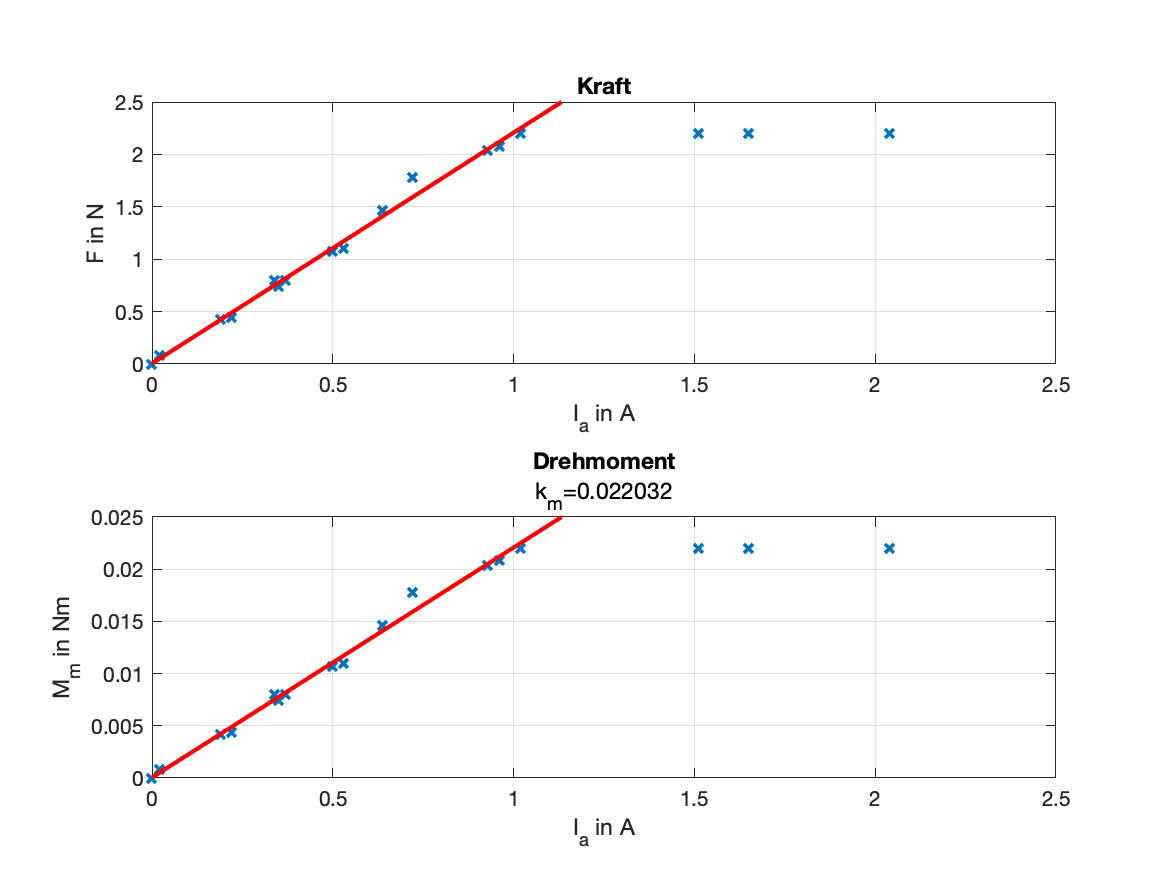
\includegraphics[width=1\textwidth]{as_labor01_1.png}
 \caption{Plot der Aufgabe 1}
 \label{fig:PlotAufgabe1}
\end{figure}
\subsubsection{Messung des Ankerwiderstand}

Im zweiten Versuch soll der Ankerwiderstand $R$ bestimmt werden.
Der Ankerwiderstand kann über das Ohm'sche Gesetz berechnet werden,
dafür ist eine Matrix mit den gemessenen Messwerten der Spannungen
und Ströme gegeben.

Da mit den Messwerten die Ströme über den Spannungen abgebildet werden ist die
Steigung nicht der Widerstand sondern der Leitwert. Deshalb muss zur Ermittlung
des Ankerwiderstand noch das Reziproke des Leitwerts berechnet werden.

\begin{equation} \label{eq121}
    \begin{split}
        R&=\frac{U_a}{I_a} \Leftrightarrow G=\frac{1}{R}=\frac{I_a}{U_a}\\
        R&\simeq 3.26 \mathrm{\Omega}
    \end{split}
\end{equation}

\begin{figure}[H]
 \centering
 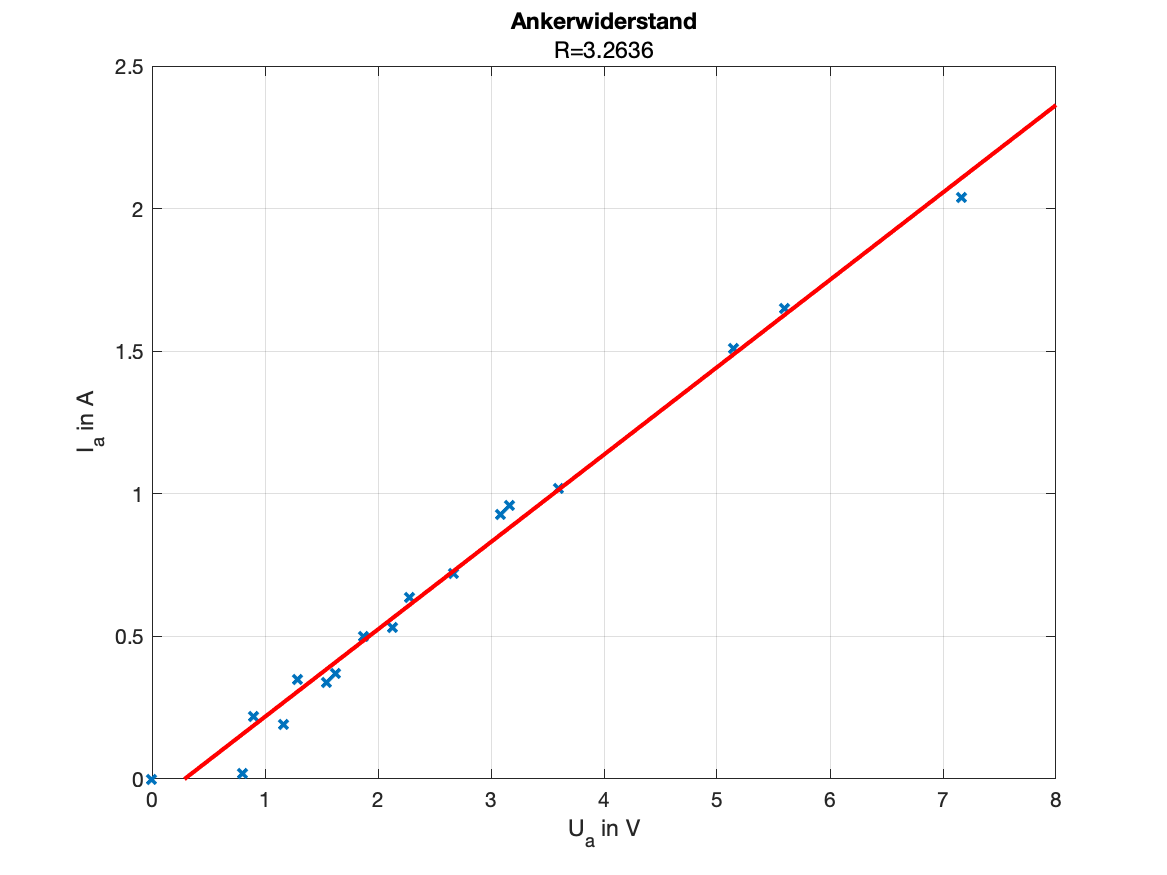
\includegraphics[width=1\textwidth]{as_labor01_2.png}
 \caption{Plot der Aufgabe 2}
 \label{fig:PlotAufgabe2}
\end{figure}
\subsubsection{Messung des Stillstandsdrehmomentes}

Im dritten Versuch soll die Konstante $k_e$ bestimmt werden. Diese
beschreibt als Proportionalfaktor den Zusammengang zwischen der
induzierten Spannung $U_i$ und der Winkelgeschwindigkeit $\omega$.

\begin{equation} \label{eq131}
    \begin{split}
        u_i(t)=k_e \cdot \omega (t)
    \end{split}
\end{equation}

Gegeben sind in dieser Aufgabe sind die Messwerte in einer Matrix. Diese
enthält die Spannungswerten von $U_a=U_i$, welche mit einem Multimeter
gemessen worden sind und den Inkrementen pro $\mathrm{ms}$ $Y$, ermittelt
durch einen Inkrementalgeber und einen Mikrocontroller.

Um $k_e$ zu bestimmen wird neben der direkt gegebenen Spannung $U_a$ auch
die Winkelgeschwindigkeit $\omega$ benötigt. Diese ist das Produkt aus
$2\pi$ und der Drehzahl $n$. Während die Winkelgeschwindigkeit angibt wie
schnell sich ein Winkel mit der Zeit um eine Achse ändert, gibt die Drehzahl
die Anzahl der Umdrehungen in einer Zeitspanne an.

\begin{equation} \label{eq132}
    \begin{split}
        k_e = \frac{U_a}{\omega}= \frac{U_a}{2 \pi n}
    \end{split}
\end{equation}

Die gemessen Inkremente pro Zeit müssen daher umgerechnet werden. Diese
wurden mit dem C167 Mikrocontroller mit einer Abtastzeit $T=1\mathrm{ms}$
aufgenommen. Der Inkrementalgeber besitzt 500 Inkremente pro Umdrehung.
Durch eine Vierfachauswertung ergeben sich $P_z=\frac{2000}{2\pi} \mathrm{\frac{INK}{rad}}$.
Dadurch ergibt sich folgender Umrechnungsfaktor $\lambda$.

\begin{equation} \label{eq133}
    \begin{split}
        \lambda = \frac{1000}{P_z} \mathrm{\frac{ms}{s} \frac{rad}{INK}}
    \end{split}
\end{equation}

Über diesen Faktor lässt sich die Drehzahl bestimmen, damit die
Winkelgeschwindigkeit und abschließend auch $k_e$.

\begin{equation} \label{eq133}
    \begin{split}
        n &= \lambda \cdot Y \qquad \text{in} \mathrm{\frac{rad}{s}}\\
        \omega &= 2 \pi \lambda \cdot Y \qquad \text{in} \mathrm{\frac{rad}{s}}\\
        k_e &= \frac{U_a}{2 \pi \lambda \cdot Y}  \qquad \text{in} \mathrm{\frac{Vs}{rad}}
    \end{split}
\end{equation}

Dadurch berechnet sich $ke$ nach über das Reziproke der Steigung der Funktion
multipliziert mit dem Faktor $\lambda$.

\begin{equation} \label{eq134}
    \begin{split}
    k_e = \frac{1}{m \cdot \lambda} \simeq 0.0235 \mathrm{\frac{Vs}{rad}}
    \end{split}
\end{equation}

\begin{figure}[H]
 \centering
 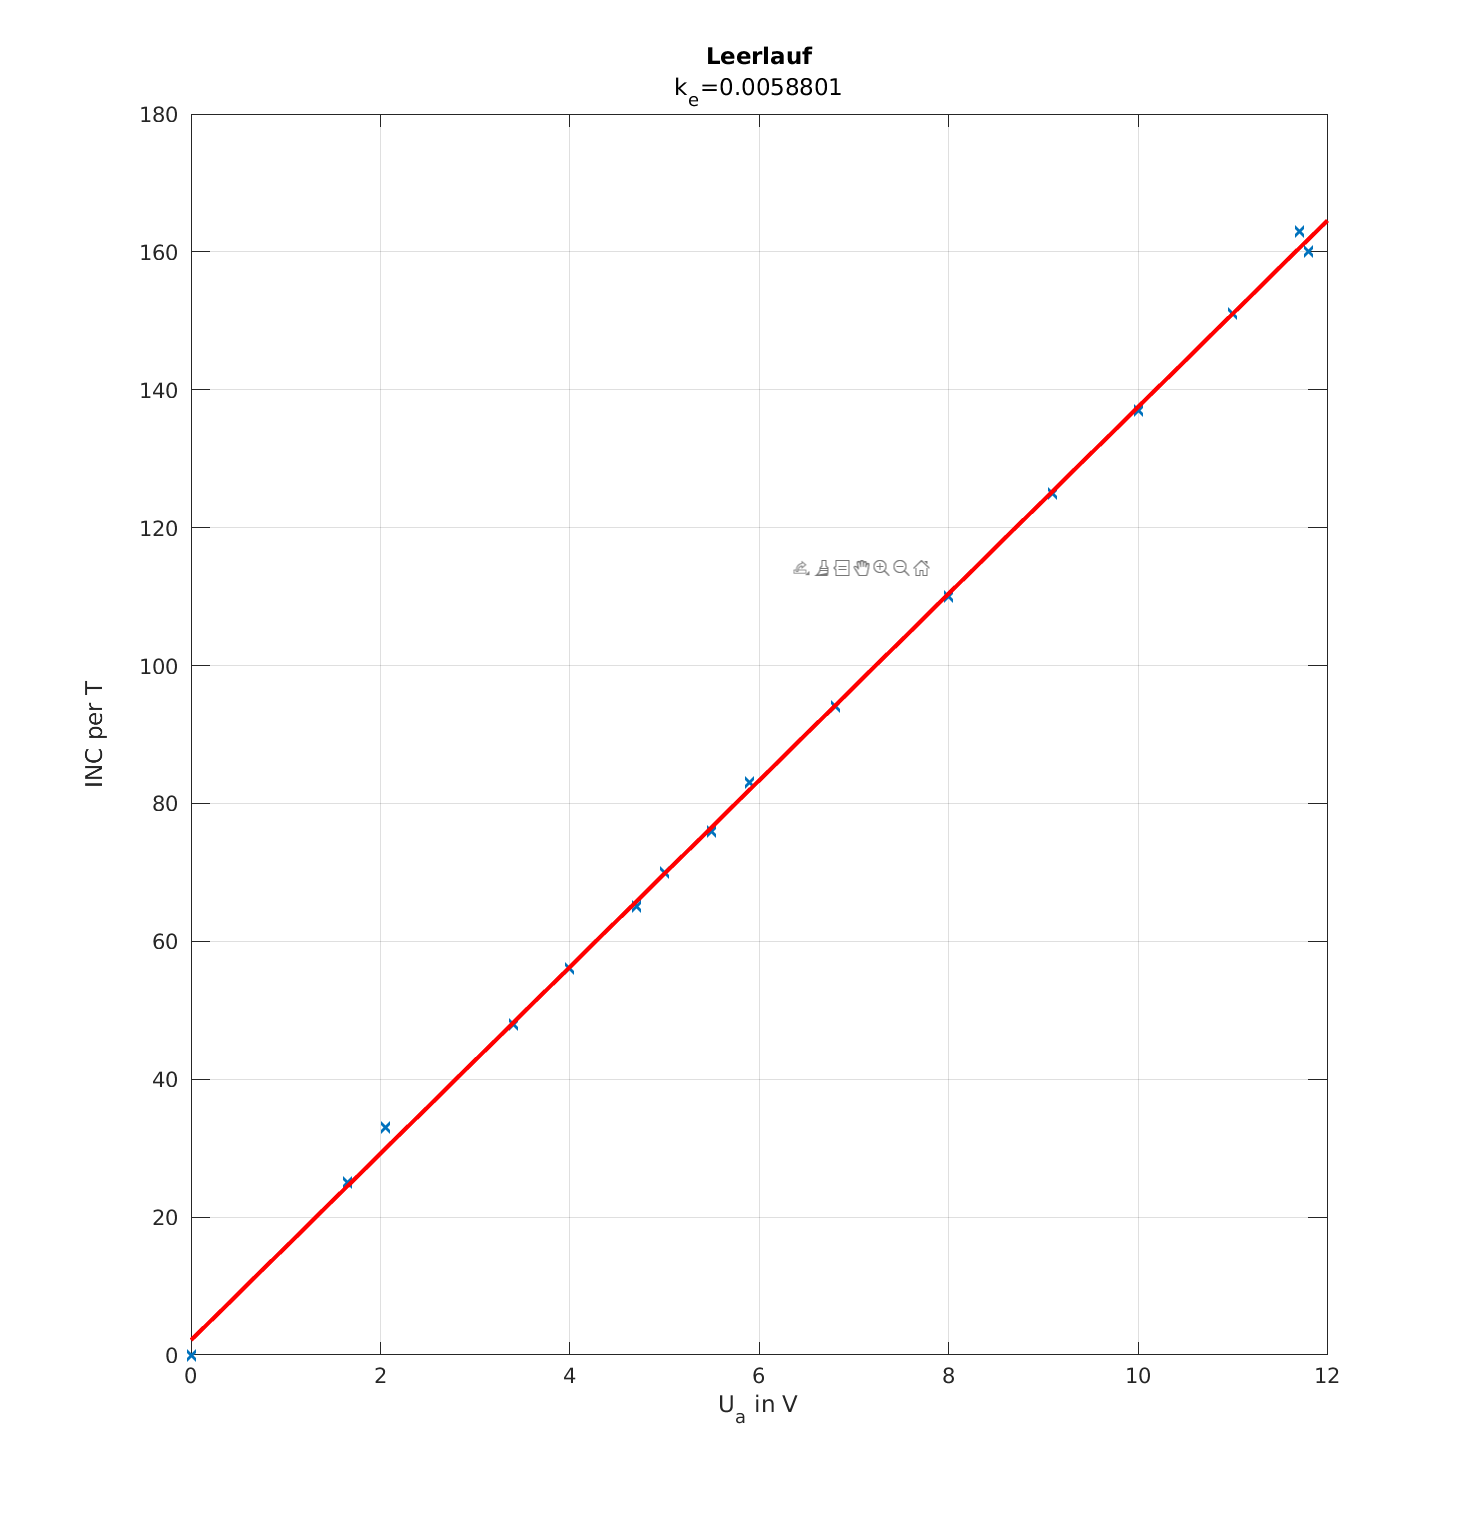
\includegraphics[width=1\textwidth]{as_labor01_3.png}
 \caption{Plot der Aufgabe 3}
 \label{fig:PlotAufgabe3}
\end{figure}
\subsubsection{Messung der Kennlinie des Verstärkers}

In der letzten Messung soll die Kennlinie des Messverstärkers ermittelt
werden und damit der Verstärkungsfaktor $A$ bestimmt werden. Dafür liegt
eine Matrix mit den Eingangsspannungen $U_e$ und den Ausgangspannungen
$U_a$ vor. Da der Verstärker ausgangsseitig bei etwa $+13.75\mathrm{V}$
und $-13.06\mathrm{V}$ in Sättigung geht, werden die jeweils ersten beiden
und die letzten beiden Messwerte für die Berechnung der Funktion nicht
betrachtet.

Der Verstärkungsfaktor $A$ ist der Quotient aus Ausgangs- und Eingangsspannung
und somit die Steigung der ermittelten Funktion.

\begin{equation} \label{eq141}
    \begin{split}
        A=\frac{U_a}{U_e}\simeq2 \mathrm{V}
    \end{split}
\end{equation}

\begin{figure}[H]
 \centering
 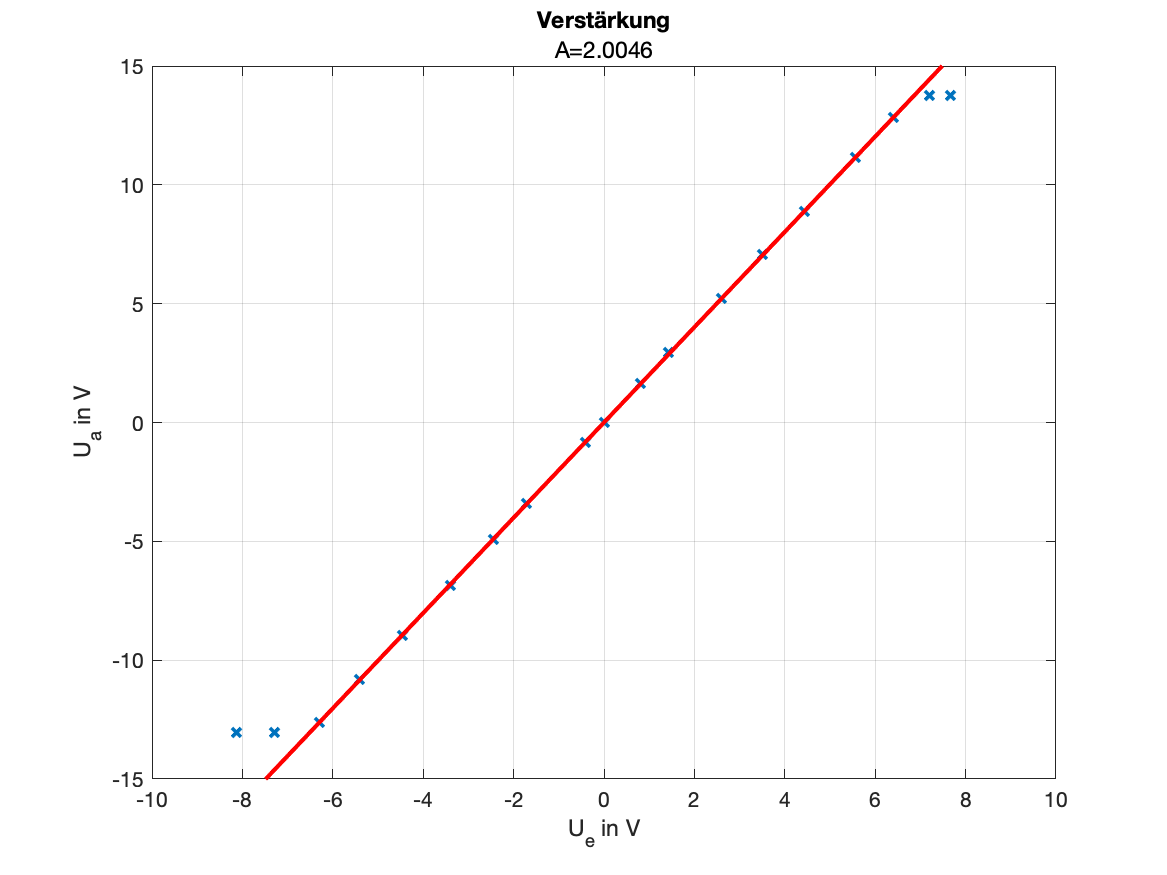
\includegraphics[width=1\textwidth]{as_labor01_4.png}
 \caption{Plot der Aufgabe 4}
 \label{fig:PlotAufgabe4}
\end{figure}
%\subsection{Zusammenfassung}
\subsection{Anhang}

\subsubsection{Aufgabenbeschreibung}
\begin{figure}[H]
    \centering
    \includegraphics[page=3, width=0.8\textwidth]{../Aufgabenstellung.pdf}
    %\caption{Aufbau der CBM-Toolchain}
    \label{fig:Aufgabenstellung A1}
\end{figure}

\begin{figure}[H]
    \centering
    \includegraphics[page=4, width=0.8\textwidth]{../Aufgabenstellung.pdf}
    %\caption{Aufbau der CBM-Toolchain}
    \label{fig:Aufgabenstellung A1}
\end{figure}

\subsubsection{Matlab Code}
\lstinputlisting[language=Matlab]{matlab/as_labor01_1.m}
\lstinputlisting[language=Matlab]{matlab/as_labor01_2.m}
\lstinputlisting[language=Matlab]{matlab/as_labor01_3.m}
\lstinputlisting[language=Matlab]{matlab/as_labor01_4.m}

%\subsubsection{Messwerte}



\end{document}
